\documentclass{beamer}
\usepackage[utf8]{inputenc}
\usepackage{subfiles}
\usepackage{lipsum}
\usepackage[algoruled, linesnumbered]{algorithm2e}
\usepackage{listings}
\usepackage{color}
\usepackage{tikz}
\usepackage{verbatim} %to use multiline comment
\usepackage{graphicx}
\usepackage{caption}

\usetheme{Madrid}

%\renewcommand\thealgorithm{}



\title[DFS]{Graph Algorithms: \newline Deapth First Search(DFS)}
\author{Nirob Arefin \inst{1} and Protik Dey \inst{2}}

\institute[BUET]{

\inst{1}
Student-ID: 1505050\\


\inst{2}
Student-ID: 1505051 \\
\vspace{5mm}

Department of Computer Science and Engineering

Bangladesh University of Engineering and Technology

}

%\section{First}


\AtBeginSection
{
\begin{frame}{Outline}
    \tableofcontents[currentsection]
\end{frame}
}

\begin{document}

\maketitle

\begin{frame}{Outline}
    \tableofcontents
\end{frame}

\section{Introduction}

\begin{frame}{Introduction}

 \begin{figure}
        \centering
        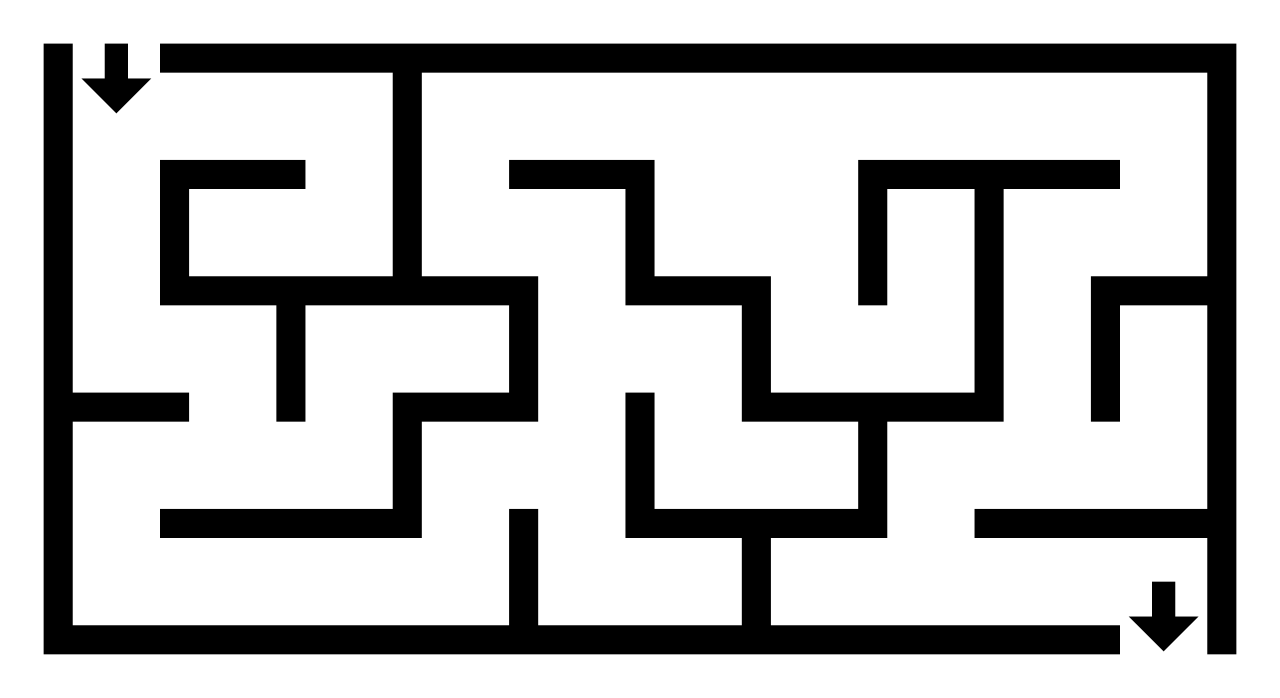
\includegraphics[width=.5\textwidth]{Pictures/maze.png}
        %\caption{Basic Classification of Human races}
        \label{fig:mazepic}
    \end{figure}
    
    \begin{itemize}
        \centering
        \item<2-> \textcolor{red}{\textbf{\huge It's a maze!!!}}
    \end{itemize}
    
    
\end{frame}

\begin{frame}{Introduction}
    \centering
    \textcolor{black}{\textbf{\Large Deapth First Search(DFS)}}
    
\end{frame}

\begin{frame}{Introduction}
    \setbeamercovered{dynamic}
    \textcolor{red}{\textbf{What is DFS?}}
    
    \begin{itemize}
        \item<2-> Algorithm for traversing graph data structures.
        \item<3-> Starts at the root node.
        \item<4-> Explores as far as possible along each branch before backtracking. 
    \end{itemize}
        
\end{frame}

\section{Pseudocode}

\begin{frame}{Pseudocode}
\begin{center}
  \subfile{Sections/Algo.tex}  
\end{center}

    
\end{frame}



\begin{frame}{Pseudocode}
    \begin{center}
        %DFS-VISIT(\displaystyle{G,u})
        \subfile{Sections/Algo2.tex}
    \end{center}
\end{frame}

\section{Example}



\begin{frame}{Example}
    
    
    
    \subfile{Sections/Figd.tex}
    
    
    
\end{frame}


\section{Complexity}


\begin{frame}{Complexity}
    \begin{columns}

    \column{0.5\textwidth}
        \begin{center}
            \subfile{Sections/Algo.tex}
        \end{center}
            

        

    \column{0.5\textwidth}
        \begin{center}
            \subfile{Sections/Algo2.tex}
        \end{center}
        

    \end{columns}
\end{frame}


\begin{frame}{Complexity}
    \setbeamercovered{dynamic}
    \begin{columns}

    \column{0.5\textwidth}
        \begin{center}
            \subfile{Sections/Algo.tex}
        \end{center}
            

        

    \column{0.5\textwidth}
        \begin{center}
            \begin{itemize}
                        \item<1-> Loop of line 2-5 take $\Theta$($V$)
                        \item<2-> Loop of line 7-10 take $\Theta(V)$
                    \end{itemize}
            %complexity is O(v+E)
        \end{center}
        

    \end{columns}
\end{frame}



    \begin{frame}{Complexity}
        \setbeamercovered{dynamic}
        \begin{columns}
        
            \column{.5\textwidth}
                \begin{center}
                    %DFS-VISIT(\displaystyle{G,u})
                    \subfile{Sections/Algo2.tex}
                \end{center}
             
             
             \column{.5\textwidth}  
             
                \begin{center}
                
                    \begin{itemize}
                        \item<1-> Loop of line 5-9 executes $|Adj[v]|$ times.
                        \item<2-> The preocedure DFS-VISIT is called exactly once for each vertex $v \epsilon V$ .
                        \item<3-> Total cost of executing lines 5-9 of DFS-VISIT is :
                        \item<4-> $$\sum_{v\epsilonV} |Adj[v]| = \Theta(E)$$
                    \end{itemize}
                    
                \end{center}
        
        \end{columns}
    
    
    
    \end{frame}
    
    
    \begin{frame}{Complexity}
        \begin{block}{Finally}
        
        
            The running time of DFS is therefore $\Theta(V+E)$
        \end{block}  
    \end{frame}
    
    
    \section{Application}
    
    \begin{frame} {Application}
        
    
        \setbeamercovered{dynamic}
        \begin{itemize}
        \item Detecting cycle in a graph
        \item<2-> Path finding
        \item<3-> Topological sorting
        \item<4-> Finding strongly connected components
        \item <5-> Solving mazes
        \end{itemize}
    
    
        
    \end{frame}
    
    \begin{frame}{Application}
    
       \textcolor{red}{\Large Topological Sorting} \pause
       
       \vspace{5mm}
       
       Procedure 
       
       \setbeamercovered{dynamic}
        \begin{itemize}
        \item<2-> call DFS(G) to compute finishing time $v.f$ for each vertex $v$
        \item<3-> as each vertex is finished,insert it onto the front of a linked list
        \item<4-> \textbf{return} the linked list of vertices
        
        \end{itemize}
       
       
        
    \end{frame}
    
   % \begin{frame}{Application}
    %    \subfile{Sections/topological1.tex}
    %\end{frame}
    
    \begin{frame}{Application}
       
        %\subfile{Sections/topological1.tex}
        \subfile{Sections/topological2.tex}
    \end{frame}
    
    \section{Acknowledgement}
    
        \begin{frame}{Acknowledgement}
            
        \begin{itemize}
            \item  Introduction to Algorithms by Thomas H.Cormen,Charles E.Leiserson,Ronald L.Rivest and Clifford Stein.
        \end{itemize}    
            
            
        \end{frame}
        
        \section{Conclusion}
        
            \begin{frame} {Conclusion}
                
                \begin{figure}
                \centering
                
\includegraphics[width=.8\textwidth]{Pictures/Q.jpg}
                %\caption{Basic Classification of Human races}
                \label{fig:mazepic}
    \end{figure}
                
            \end{frame}

\end{document}  

